\documentclass[letterpaper]{article} % DO NOT CHANGE THIS
\usepackage[submission]{aaai2027} % DO NOT CHANGE THIS
\usepackage[hyphens]{url} % DO NOT CHANGE THIS
\usepackage{graphicx} % DO NOT CHANGE THIS
\urlstyle{rm} % DO NOT CHANGE THIS
\def\UrlFont{\rm} % DO NOT CHANGE THIS
\usepackage{natbib} % DO NOT CHANGE THIS AND DO NOT ADD ANY OPTIONS TO IT
\usepackage{caption} % DO NOT CHANGE THIS AND DO NOT ADD ANY OPTIONS TO IT
\usepackage{booktabs}
\usepackage{amsmath}
\usepackage{amssymb}
\frenchspacing % DO NOT CHANGE THIS

\pdfinfo{
/TemplateVersion (2027.1)
}

\setcounter{secnumdepth}{1}

\title{TerraState: A Testable Predictive-State World Model for Weather-Driven Land-Surface Forecasting}
\author{Anonymous Submission}
\affiliations{}

\begin{document}

\maketitle

\begin{abstract}
High-resolution satellite time series are a primary tool for monitoring
vegetation, agriculture, and ecosystem response. Forecasting from these
series is increasingly formulated as a weather-driven task: predicting
future land-surface observations from cloud-obscured image histories and
meteorological drivers. Yet such models are primarily evaluated by
fixed-horizon pixel accuracy, which cannot establish whether an internal
representation functions as a forecast-bearing, weather-responsive
predictive state. An accurate forecaster may still ignore the weather
forcing, collapse toward persistence, or expose a latent state that does
not actually carry the forecast---failures that standard error metrics
cannot detect. We introduce \textbf{TerraState}, a testable
predictive-state world model. TerraState infers a spatial predictive state
from cloud-masked histories. A shared transition advances this state under
future weather, geography, and elapsed time, and a state readout converts
the advanced state into an explicit contribution to the final forecast.
Rather than treating architecture alone as evidence that a world state
exists, TerraState makes its predictive-state claim falsifiable through
state-contribution removal, a supporting identity-transition control, and
matched interventions comparing actual future weather with matched-donor
and normalized-mean weather. On GreenEarthNet under temporal distribution
shift, TerraState retains useful forecasting skill; state removal degrades
validation and OOD-t performance, and actual weather yields lower
complete-window loss than both controls on a frozen heat--drought subset.
\end{abstract}

\section{Introduction}

High-resolution Earth-observation (EO) time series support localized
monitoring of vegetation, agriculture, and ecosystem response. Forecasting
future land-surface observations requires combining sparse, cloud-obscured
satellite histories with past meteorology, static geography, and supplied
future weather. EarthNet2021 formalized this setting as guided video prediction
from past Sentinel-2 observations, topography, and future meteorology
\cite{requenamesa2021earthnet}; GreenEarthNet refined it with
vegetation-focused cloud masking, temporal-distribution-shift evaluation, and
high-resolution weather-conditioned forecasting \cite{benson2024multimodal}.
We study this task from a predictive-state world-modeling perspective: a model
must summarize incomplete observations and represent how the observed surface
may evolve under future forcing.

\begin{figure*}[t!]
\centering
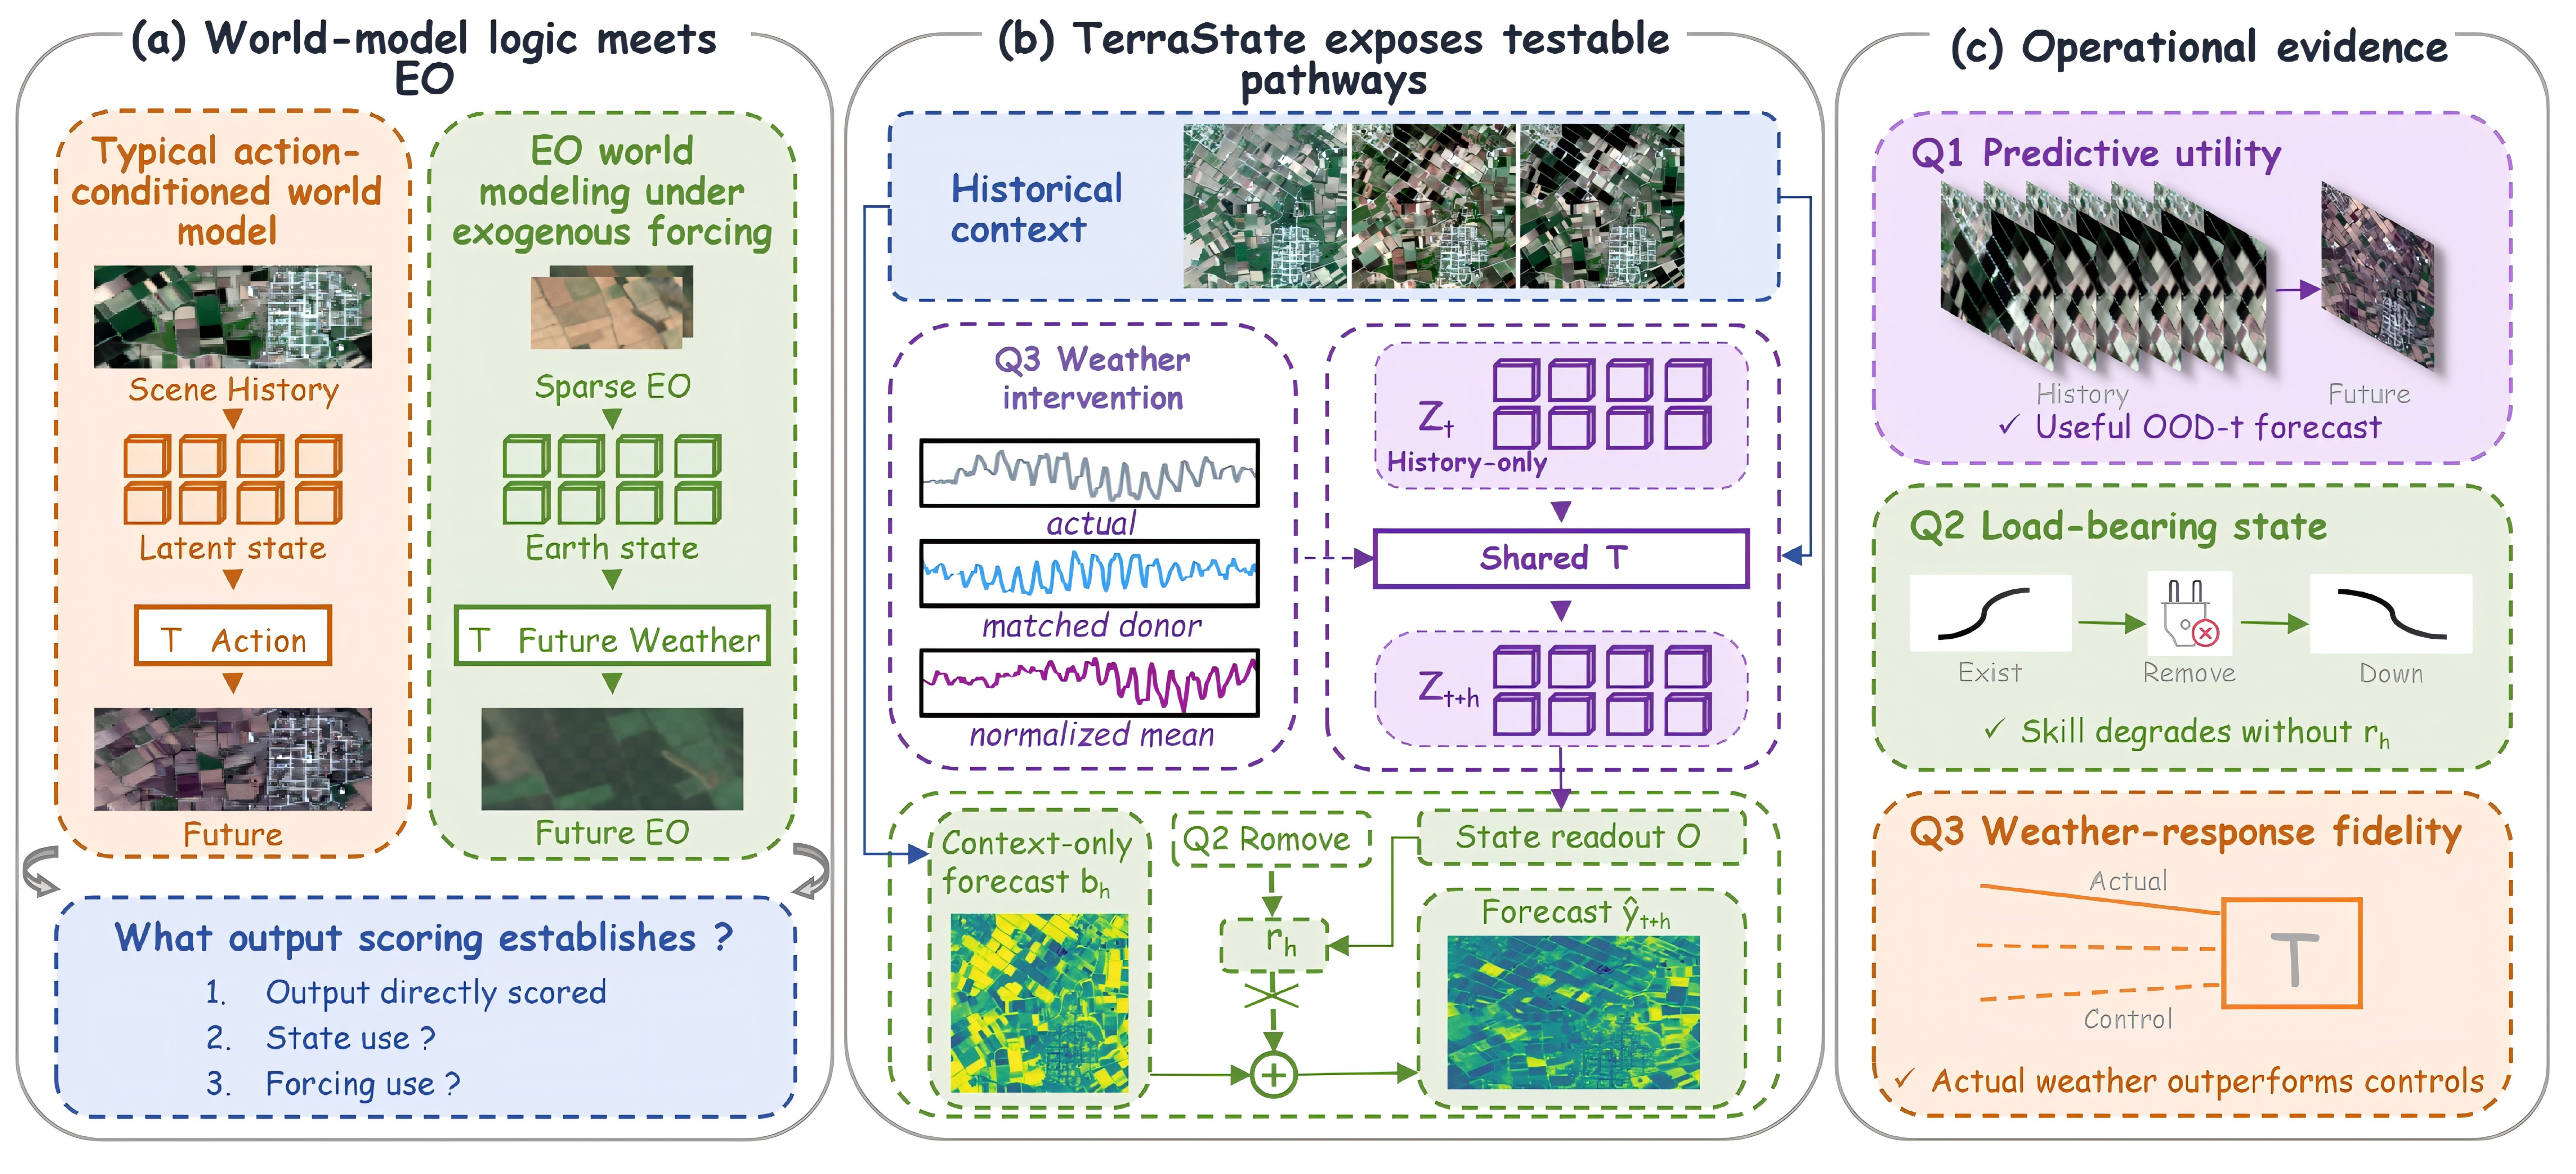
\includegraphics[width=0.98\textwidth]{figures/terrastate_concept_overview_author_layout_20260729.png}
\caption{Conceptual overview of TerraState's testable EO world-modeling
contract. (a) Action-conditioned world-model logic maps to EO modeling under
exogenous weather forcing, while output scoring alone leaves internal state and
forcing use untested. (b) TerraState exposes a history-only predictive state,
shared weather-conditioned transition, state readout, and intervention
interfaces. (c) Q1--Q3 provide evidence for predictive utility, state
contribution, and weather-response fidelity.}
\label{fig:contract}
\end{figure*}

Weather-conditioned EO forecasters have improved the quality of predicted
observations. Within standard EO forecasting benchmarks, however, the primary
evidence remains output accuracy over a fixed forecast window
\cite{requenamesa2021earthnet,benson2024multimodal}. Such accuracy shows whether outputs resemble
observations, but cannot by itself establish whether an internal state
contributes to those outputs or whether future meteorology advances that state.
A predictor may bypass its latent state, use weather only weakly, or behave as
a one-shot mapping; accurate outputs can also coexist with temporally
disordered latent representations \cite{yang2026latenttsf}.

Predictive-state representations characterize state through future observables
rather than an assumed hidden physical variable
\cite{littman2001predictive}. This motivates a concrete question:
\emph{can an EO forecaster expose a predictive state that both carries the
forecast and mediates a faithful response to future weather?} Accordingly, we
introduce TerraState, a testable predictive-state world model for
weather-driven EO forecasting. TerraState makes these properties empirical
claims rather than consequences of naming a hidden representation. Its scope
is deliberately narrower than recovering a complete physical state or
building a causal or general-purpose generative simulator.

Figure~\ref{fig:contract} summarizes the resulting model. TerraState infers a
spatial predictive state from cloud-masked EO history, past meteorological
observations, and static geography. A shared transition advances that state
under supplied future weather, geography, and elapsed time. The state readout
turns the advanced state into an explicit forecast contribution that is added
to a context-only prediction, so state use is exposed in the final output
rather than only in a hidden layer. During training, a frozen representation
of observed future EO anchors the transitioned state without exposing future
observations at inference. After training, state-contribution removal tests
forecast relevance, while weather-path substitution tests the response to
supplied forcing without retraining.

On GreenEarthNet OOD-t, TerraState obtains \(R^2=0.569\) and
\(\mathrm{RMSE}=0.151\), retaining useful forecasting skill under temporal
shift. Removing the state contribution reduces performance on both validation
and OOD-t, with paired confidence intervals excluding zero. On the frozen
matched subset, actual future weather yields lower masked loss over the
complete 20-step forecast window than matched-donor and normalized-mean
controls. Together, these results support a load-bearing, weather-responsive
predictive state under the evaluated protocol.

Our contributions are:
\begin{itemize}
    \item We frame weather-driven EO world modeling around a falsifiable
    question: whether a history-derived predictive state both contributes to
    the forecast and mediates its response to future meteorological forcing.
    \item We introduce TerraState, which combines an explicit state-mediated
    forecast path, a shared weather-conditioned transition, and future-state
    anchoring from observed future EO during training.
    \item We evaluate the same trained model at three levels: useful
    temporal-shift forecasting, load-bearing state contribution on validation
    and OOD-t, and greater complete-window fidelity under actual weather than
    under matched-donor and normalized-mean controls.
\end{itemize}

\section{Related Work}

\paragraph{Weather-conditioned EO forecasting.}
Weather-conditioned EO forecasting predicts future land-surface observations
from satellite histories, meteorology, and geographic context. EarthNet2021
formalized this guided video-prediction setting, and GreenEarthNet/Contextformer
refined it for vegetation dynamics and temporal shift
\cite{requenamesa2021earthnet,benson2024multimodal}. Deterministic methods use
recurrent, convolutional, or transformer predictors
\cite{shi2015convlstm,wang2017predrnn,gao2022simvp,gao2022earthformer}, whereas
video-diffusion models represent multiple plausible futures
\cite{voleti2022mcvd,zhao2024vegediff}. ViT-Koop advances a compressed EO state,
and prior weather-response analysis perturbs meteorological inputs at the output
level \cite{shinohara2025vitkoop,diaconu2022weather}. Across these strands,
evidence centers on forecast outputs, with some studies also analyzing weather
response or learned representations. This leaves a narrower question about
whether an explicit internal state participates in the prediction path and
responds to supplied weather.

\paragraph{World models: latent dynamics to interactive environments.}
World-model research supplies the broader context for this shift from output
prediction to explicit internal state. A control-oriented lineage compresses
observations and learns latent transitions for rollout, planning, or imagination
\cite{ha2018worldmodels,hafner2019planet,hafner2020dreamer}. MuZero predicts
planning-relevant policy, value, and reward \cite{schrittwieser2020muzero}. IRIS
learns an agent inside a tokenized world model, whereas Genie learns
action-controllable environments from video
\cite{micheli2023iris,bruce2024genie}. Drive-OccWorld connects
action-conditioned occupancy forecasting to driving planning
\cite{yang2025driveoccworld}. These examples share a
state--transition--prediction structure but optimize different downstream
objectives, motivating a task-specific account of predictive state in EO.

\paragraph{EO world models and forcing-conditioned simulation.}
In EO, this shared structure must be specialized to partially observed
geospatial processes under external environmental drivers. Recent preprints
make this connection explicit. EO-WM structures weather forcing for
probabilistic EO forecasting and output-response diagnostics
\cite{luo2026eowm}. VegSim rolls a latent vegetation state under user-specified
weather for scenario-conditioned simulation \cite{iele2026vegsim}. A
cloud-aware model instead predicts future observation availability rather than
land-surface pixels \cite{albughdadi2026observability}. Here, future weather is
an exogenous input for forecasting EO observations rather than the prediction
target itself. Complementing these objectives, TerraState examines whether the
state used by a weather-conditioned EO forecast makes a removable contribution
and whether actual forcing yields greater complete-window fidelity than frozen
controls.

\paragraph{Predictive states and testability.}
Predictive-state work asks how internal state is defined, supervised, and
evaluated. Classical predictive-state representations define state through
future observables, and Predictive-State Decoders explicitly supervise
recurrent states to predict those observables
\cite{littman2001predictive,venkatraman2017predictivestate}. I-JEPA and V-JEPA
learn predictive representations without reconstructing raw pixels
\cite{assran2023ijepa,bardes2024vjepa}. LatentTSF shows that accurate forecasts
can coexist with temporally disordered latents \cite{yang2026latenttsf}, while
PLSM constrains action effects in a control setting \cite{saanum2024simplifying}.
In automaton-governed generative-model settings, dedicated evaluation further
reveals incoherence missed by standard diagnostics \cite{vafa2024evaluating}.
Together, these works motivate an EO-specific test: output accuracy alone
cannot establish that an exposed state carries prediction or mediates weather
forcing. Section 3 therefore constructs TerraState around an on-path predictive
state, a shared weather-conditioned transition, and state-removal and
weather-control interfaces that make this bounded claim testable.

\section{Method}

\subsection{Problem Formulation and Model Overview}

Weather-driven Earth-observation (EO) world modeling seeks to represent how
the land surface evolves from incomplete satellite histories under future
meteorological forcing. We formulate this task around a predictive state
inferred from observation history, advanced by the supplied meteorological
forcing, and decoded into future observations.

Accordingly, we introduce TerraState as a testable predictive-state world
model. TerraState differs from a conventional EO predictor by making the
predictive state's contribution explicit in the final forecast. A history
operator and projector construct $z_t$, and a shared transition advances it
under the ordered future-weather prefix, static geography, and forecast
horizon. A state readout decodes the advanced state into the state-mediated
forecast contribution $r_h$. TerraState combines $r_h$ with the context-only
forecast $b_h$.

At forecast issue time $t$, let
$\mathcal H_t=\{(x_i,m_i,\tau_i)\}_{i=1}^{C}$ denote cloud-obscured optical
history with validity mask $m_i$ and acquisition time $\tau_i$. Historical
weather is $u_{\leq t}^{\rm past}$, and the ordered $H$-step future sequence is
$u_{t+1:t+H}$; $g$ denotes static geography and $y_{t+1:t+H}$ the targets. Let
$\widetilde{\mathcal C}_t=(\mathcal H_t,u_{\leq t}^{\rm past},g)$ and query
$h\in\{1,\ldots,H\}$. TerraState realizes this formulation through:
\begin{equation}
\begin{aligned}
(b_{1:H},e_t)&=q_\theta(\widetilde{\mathcal C}_t),\\
z_t&=P_\rho(e_t),\\
z_{t+h}&=T_\psi(z_t,u_{t+1:t+h},g,h),\\
r_h&=O_\omega(z_{t+h}),\\
\widehat y_{t+h}&=b_h+r_h .
\end{aligned}
\label{eq:contract}
\end{equation}
Here, $q_\theta$ emits context-only forecasts $b_{1:H}$ and spatial tokens
$e_t$, $P_\rho$ constructs $z_t$, and $T_\psi$ advances it to $z_{t+h}$.
The readout $O_\omega$ decodes the horizon-specific spatial forecast
contribution $r_h$ from the advanced state.

By construction, $q_\theta$ has access only to observation history, past
weather, and static geography; it receives neither future EO observations nor
future meteorological forcing. The future-weather sequence enters only through
$T_\psi$, which directly advances the same $z_t$ for each $h$. The explicit
addition of $r_h$ supports separate tests of whether the state carries
predictive information and whether the forecast responds to the supplied
weather. This formulation treats $z_t$ as a predictive representation used by
the forecast, rather than claiming recovery of a complete physical state or a
causal simulator.

\subsection{TerraState Architecture}

This subsection details the inference architecture that realizes
Equation~\ref{eq:contract}. The history module produces a context-only
forecast and a spatial predictive state. A shared transition advances that
state under future meteorological forcing, and a state readout converts the
advanced state into an additive forecast contribution. Figure~\ref{fig:architecture}
illustrates these three modules.

\begin{figure*}[t]
\centering
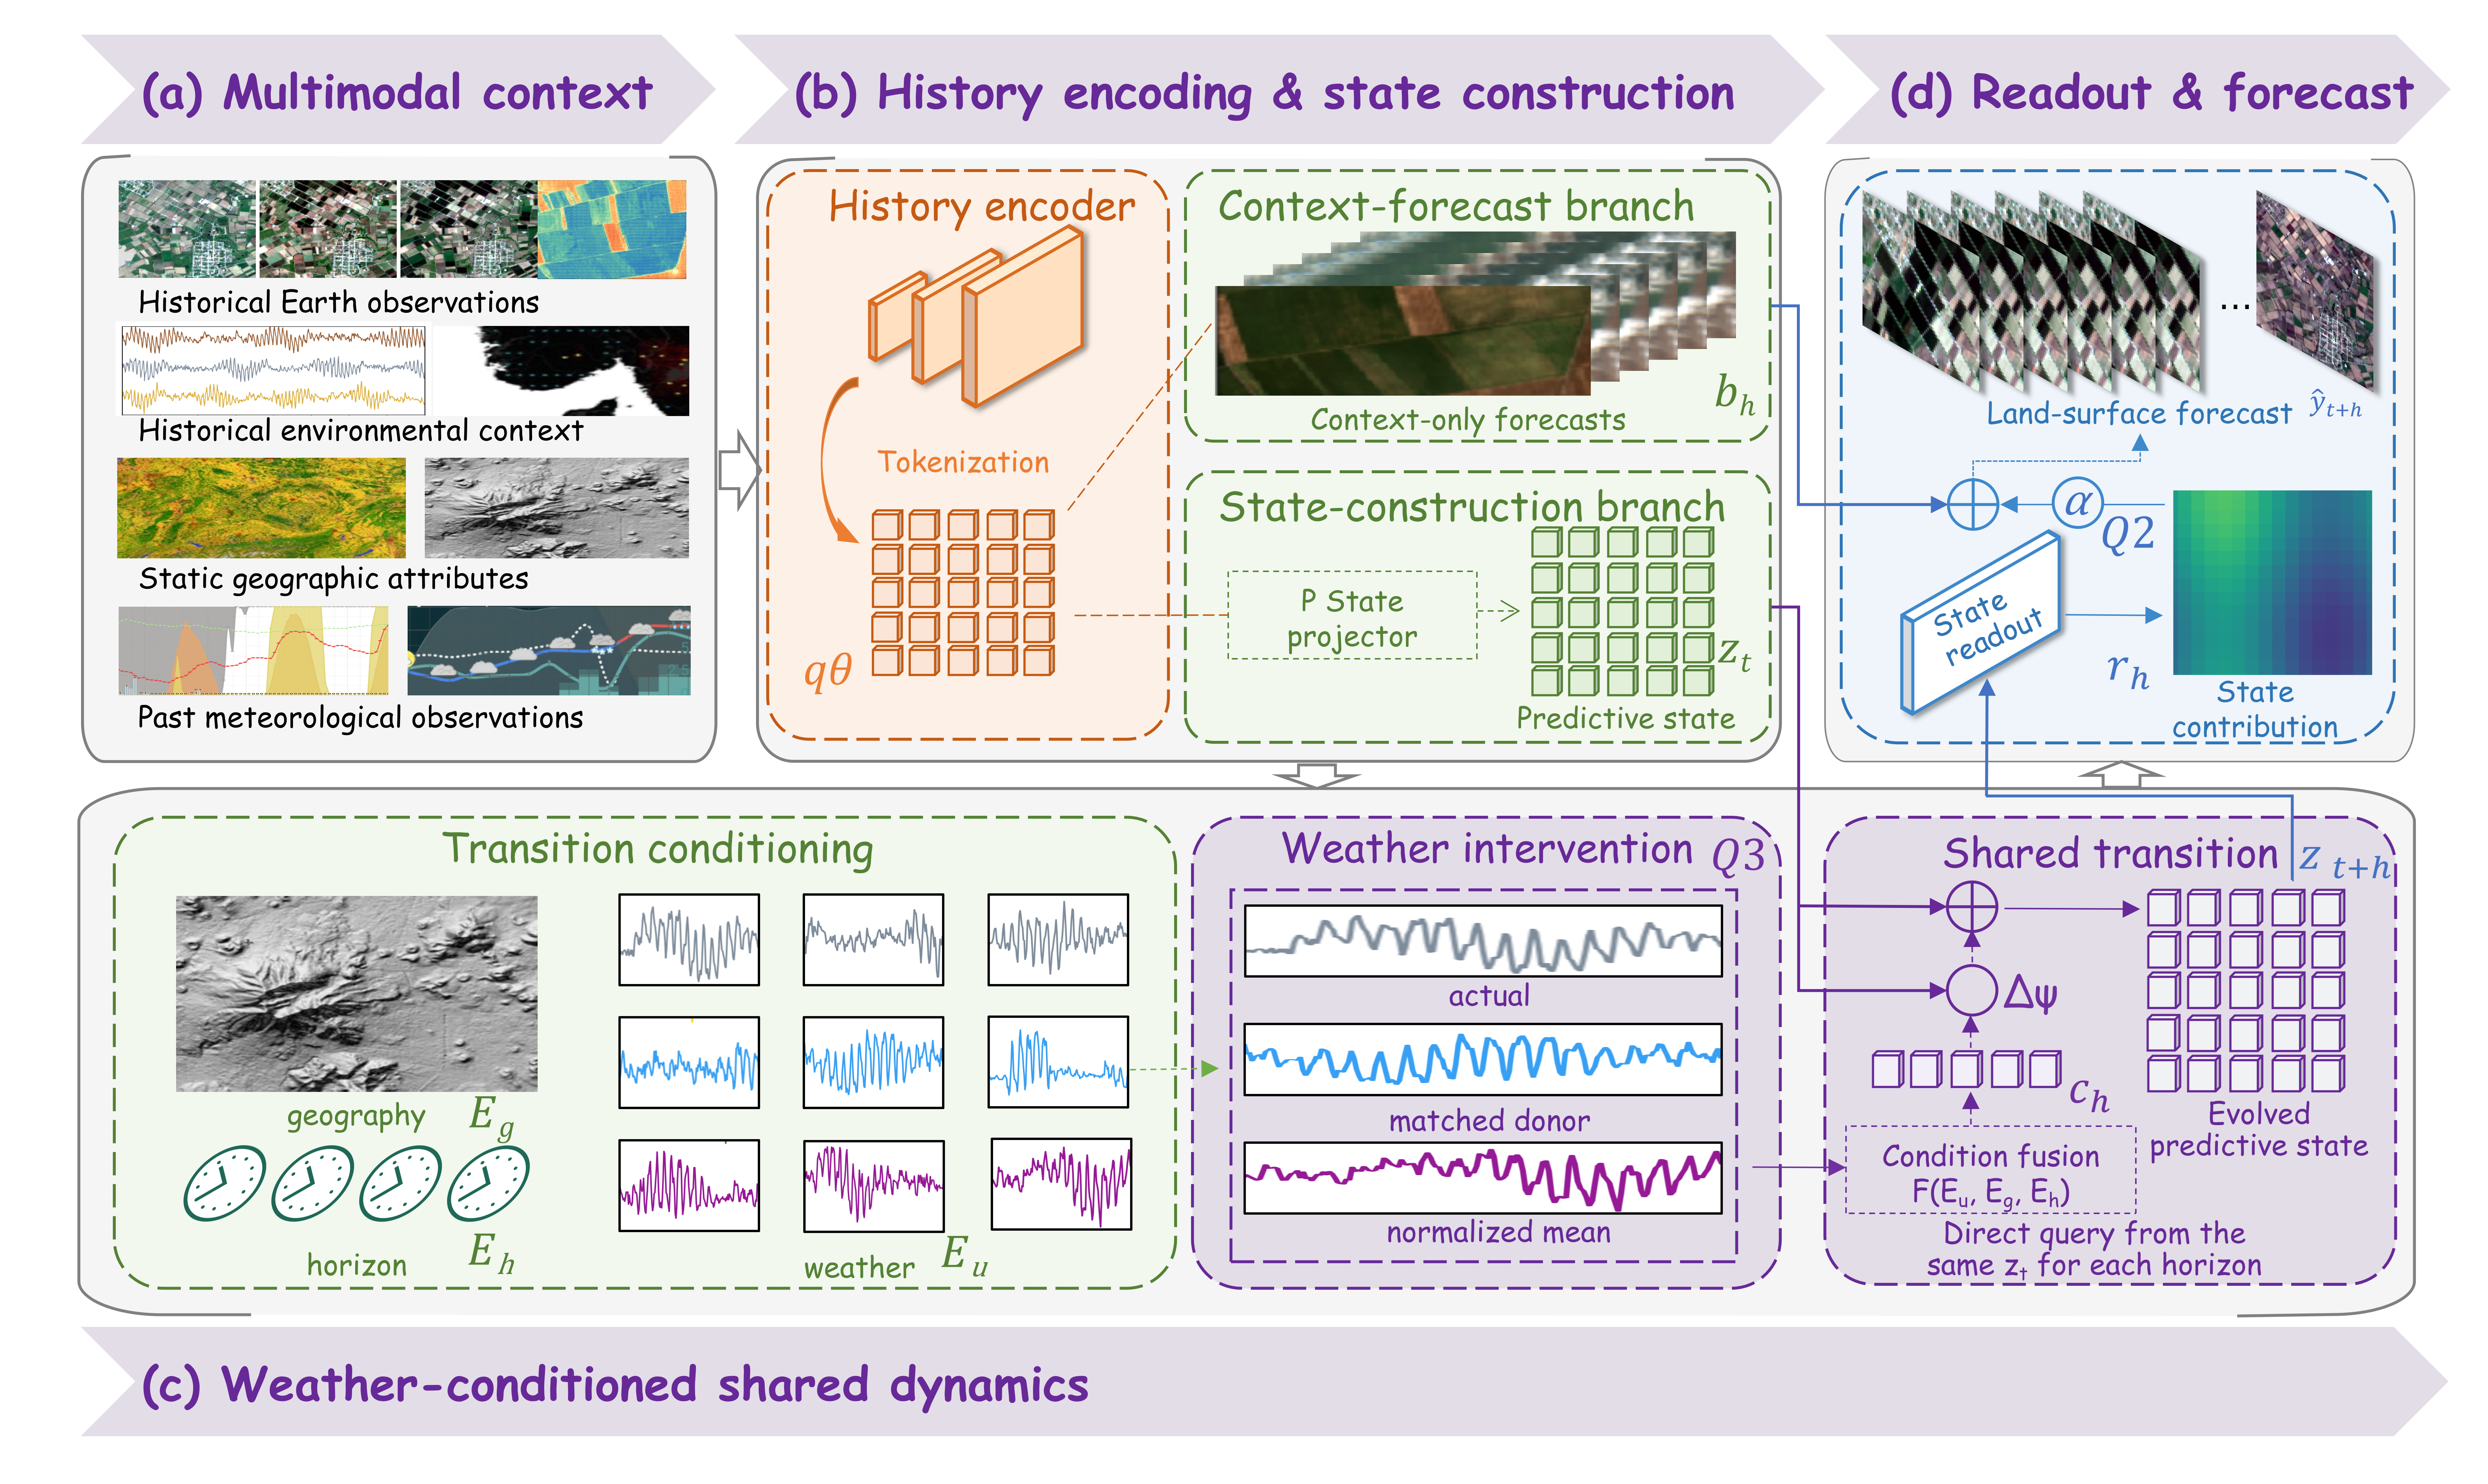
\includegraphics[width=\textwidth]{figures/terrastate_architecture_fig2_author_layout_20260729.png}
\caption{TerraState architecture and intervention interfaces. The diagram
organizes multimodal historical context, history encoding and predictive-state
construction, a shared weather-conditioned transition, and state readout into
the final forecast. Cloud-masked EO history, past meteorological observations,
and static geography form the context for the history encoder; future
meteorological forcing enters the shared transition together with geography
and the queried horizon. The transitioned state is read out as an explicit
state contribution and combined with the context-only forecast. Q2 removes
this state contribution, while Q3 holds the historical context fixed and
replaces actual future weather with season-, geography-, and quality-matched
donor weather or normalized-mean weather. These interventions test state
contribution and forecast-window response fidelity, not composition or causal
effects.}
\label{fig:architecture}
\end{figure*}

\begin{figure}[t]
\centering
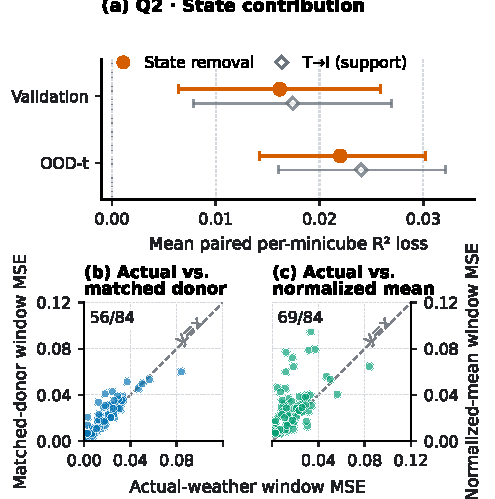
\includegraphics[width=0.79\columnwidth]{../figure_workspace/export/fig3_behavior_singlecol_aaai_cropped.pdf}
\caption{State and weather interventions. (a) Per-minicube $\Delta R^2$ for
state removal (filled, primary) and $T\!\rightarrow I$ (open, supporting),
with paired-bootstrap 95\% CIs. (b,c) Complete 20-step-window masked MSE for
actual versus matched-donor and normalized-mean weather on 84 frozen pairs.
Above-diagonal points favor actual weather; 56/84 and 69/84 are descriptive.}
\label{fig:behavior}
\end{figure}

\paragraph{Historical Context and Spatial Predictive State.}
Historical context must support both the context-only forecast and the state
that future forcing advances. In one forward pass, the history operator $q_\theta$
processes cloud-masked EO history, past meteorological observations, and
static geography, and outputs both $b_{1:H}$ and spatial context tokens $e_t$.
The projector maps the tokens at the final historical time to
$z_t=P_\rho(e_t)\in\mathbb R^{N\times d}$. Each of the $N$ tokens corresponds
to a spatial patch, preserving the patch-level organization required by the
later state readout. The context-only forecast and predictive state are
therefore derived from the same historical context but remain distinct
outputs. We instantiate $q_\theta$ with a pretrained PVT
v2/Contextformer backbone \cite{wang2022pvtv2,benson2024multimodal}.

\paragraph{Shared Weather-Conditioned Transition.}
Future weather conditions the predictive-state transition through its ordered
prefix. A shared GRU weather encoder summarizes each prefix, while separate
encoders represent patch-wise static geography and the queried horizon. For
spatial patch $i\in\{1,\ldots,N\}$,
\begin{equation}
d_h=E_u(u_{t+1:t+h}),\qquad
c_{h,i}=F\!\left([d_h;E_g(g)_i;E_h(h)]\right).
\label{eq:condition}
\end{equation}
The weather code $d_h$ and horizon embedding $E_h(h)$ are broadcast across
patches, whereas $E_g(g)_i$ retains patch-wise geographic variation. The
resulting condition therefore varies with both horizon and spatial patch.
It drives the residual state update
\begin{equation}
z_{t+h,i}
=z_{t,i}+\Delta_\psi\!\left(
[\operatorname{LN}(z_{t,i});c_{h,i}]\right).
\label{eq:transition}
\end{equation}
The weather encoder, geography encoder, condition-fusion network, and
transition parameters are shared across patches and horizons; the condition
values themselves need not be spatially identical. For each queried $h$, the
model applies the residual transition once to the same $z_t$, using
$u_{t+1:t+h}$ and the corresponding horizon code. It does not recursively
roll out $z_t\!\to z_{t+1}\!\to\cdots$. Separating historical state
construction from future forcing isolates future meteorological forcing within
state evolution.

\paragraph{State Readout and Additive Forecast.}
To connect the transitioned state to observable predictions, the state
readout $O_\omega$ maps each spatial token to a local $4\times4$ patch and
reassembles the patches into the raster contribution $r_h$. This contribution
is added to the context-only forecast:
\begin{equation}
r_h=O_\omega(z_{t+h}),\qquad
\widehat y_{t+h}=b_h+\alpha r_h,\quad \alpha\equiv1.
\label{eq:closure}
\end{equation}
The coefficient $\alpha$ remains fixed throughout training and inference.
The additive design isolates a distinct state-mediated forecast contribution
for direct evaluation, while retaining the context-only forecast as its
matched reference.

\subsection{Future-Anchored State Learning}

\paragraph{Training Identities and Purpose.}
To align the transitioned state with observed future evidence without exposing
future EO at inference, training separates the deployable TerraState student
from two frozen reference branches. An exact full-model warm start from a
forecasting precursor initializes the student, which follows the inference chain in
Equation~\ref{eq:contract}. An independent full-weather \emph{KD teacher} reads
the EO observation history, past weather, static geography, and the complete future-weather
sequence, but no future EO, and produces a stopped forecast target. The
\emph{future-state target encoder} is a training-start frozen copy of the
student's $q_\theta$ and $P_\rho$ and constructs the latent target described
below. Both reference branches remain frozen, gradients update only student
parameters enabled by the training schedule, and neither branch is invoked at
inference.

\paragraph{Forecast Objectives.}
Two forecast objectives train the student against observed NDVI and regularize
it toward the full-weather teacher. Let $b$, $h$, and $p$ index minicubes,
forecast horizons, and raster pixels. We use $c_{bhp}$ for the clear-observation
indicator, $v_{bp}$ for the vegetation indicator, and
$a_{bp}=\max_h\mathbf 1[\widehat y_{bhp}\ne-1]$ for prediction validity.
With $\widehat y^{\rm tea}$ denoting the teacher forecast,
\begin{equation}
\begin{aligned}
\bar\ell^{\rm GT}_{bp}
&=\frac{\sum_h c_{bhp}(\widehat y_{bhp}-y_{bhp})^2}
{\sum_h c_{bhp}+\epsilon_{\rm pix}},\\
\mathcal L_{\rm GT}
&=\frac{\sum_{b,p}v_{bp}a_{bp}\bar\ell^{\rm GT}_{bp}}
{\sum_{b,p}v_{bp}a_{bp}+\epsilon_{\rm GT}},\\
\mathcal L_{\rm KD}
&=\frac{\sum_{b,h,p}c_{bhp}v_{bp}
(\widehat y_{bhp}-\operatorname{sg}[\widehat y^{\rm tea}_{bhp}])^2}
{\sum_{b,h,p}c_{bhp}v_{bp}+\epsilon_{\rm KD}}.
\end{aligned}
\label{eq:forecastlosses}
\end{equation}
Thus, $\mathcal L_{\rm GT}$ first normalizes each pixel by its clear horizons
and then averages over vegetation pixels with valid predictions.
$\mathcal L_{\rm KD}$ instead forms one global mean over clear vegetation
time--pixel elements; its stop-gradient target regularizes the student without
updating the teacher.

\paragraph{Future-State Representation Target.}
The future-state objective anchors the terminal transitioned state to a
representation constructed from observed future EO. Define
$\mathcal C^*_{t+H}$ as the observed all-frame EO sequence with its recorded
masks, including future frames, together with past weather and static
geography; future weather is zeroed in this branch. The frozen copy runs the
history operator in all-frames-visible encoding mode, with every temporal
position supplied together with its recorded mask. It then selects the
terminal spatial token and applies its frozen projector. Only the terminal
future-state target is formed. For terminal spatial patch $i$,
\begin{equation}
\begin{aligned}
z^*_{t+H,i}
&=\operatorname{sg}\!\left[
P_{\rho^0}\!\left(
q_{\theta^0}(\mathcal C^*_{t+H})_{t+H,i}\right)\right],\\
\ell_i
&=1-\cos\!\left(
\operatorname{LN}(z_{t+H,i}),
\operatorname{LN}(z^*_{t+H,i})\right),\\
\mathcal L_{\rm FS}
&=\frac{\sum_i m_i\ell_i}{\sum_i m_i+\epsilon_{\rm FS}},
\end{aligned}
\label{eq:futurestate}
\end{equation}
where $(\theta^0,\rho^0)$ denotes the training-start frozen copy and
$\operatorname{sg}$ stops target gradients; $i$ indexes terminal patches
across the batch. The mask $m_i$ requires the terminal $4\times4$ patch to be
fully clear and to contain at least one vegetation pixel. Future EO is used
only to construct a stopped, training-only target; it is never an input to the
student forecast or inference graph.

\paragraph{Total Objective and Inference Boundary.}
The complete training objective is
\begin{equation}
\mathcal L
=\mathcal L_{\mathrm{GT}}
+0.5\,\mathcal L_{\mathrm{KD}}
+\lambda_s\,\mathcal L_{\rm FS}.
\label{eq:total}
\end{equation}
The KD teacher and future-state target encoder are discarded after training,
leaving the student inference graph unchanged. Future-state alignment shapes
what the transitioned state represents; the following interfaces test whether
that state affects forecasts and responds to supplied weather.

\subsection{Testable Predictive-State Interfaces}

We therefore define two post-training interfaces on the same frozen
TerraState model. Each interface changes only a designated part of the forward
computation, requires no retraining, and introduces no additional objective.

\paragraph{State-contribution intervention.}
This interface tests whether the explicit state contribution improves the
forecast. Immediately before the addition in Equation~\ref{eq:closure}, we
temporarily set $\alpha=0$, yielding
$\widehat y_{t+h}^{\,\mathrm{remove}}=b_h$. The frozen model, evaluated sample,
historical context, state construction, transition, readout, and ground-truth
forecast window remain fixed. We call the state-mediated contribution
\emph{load-bearing} when removing $r_h$ degrades paired forecast quality in
the expected direction and the prespecified uncertainty interval excludes
zero. Section~4 specifies the forecast metric and uncertainty analysis.
Replacing $T_\psi$ by the identity is only a supporting diagnostic of
transition involvement; it is not part of the load-bearing definition because
the identity substitution presents $O_\omega$ with states outside its trained
input distribution.

\paragraph{Controlled weather-path substitution.}
This interface tests whether future weather affects the forecast through the
state-mediated path and whether that response has forecast-window fidelity.
It fixes the frozen model, evaluated sample, historical context, $b_{1:H}$,
$z_t$, static geography, queried horizon, readout, and ground-truth forecast
window. Only the future-weather sequence supplied to $T_\psi$ is substituted
among actual weather, matched-donor weather, and normalized-mean weather:
\begin{equation}
\begin{aligned}
\widehat y_{t+h}(u)
&=b_h+O_\omega\!\left(
T_\psi(z_t,u_{t+1:t+h},g,h)\right),\\
\Delta L_{\rm ctrl}
&=\mathcal L_{\rm win}
\!\left(\widehat{\mathbf y}(u^{\rm ctrl}),\mathbf y\right)\\
&\quad-\mathcal L_{\rm win}
\!\left(\widehat{\mathbf y}(u^{\rm act}),\mathbf y\right),
\end{aligned}
\label{eq:interfaces}
\end{equation}
where $u\in\{u^{\rm act},u^{\rm don},u^{\rm mean}\}$,
$\mathrm{ctrl}\in\{\mathrm{don},\mathrm{mean}\}$, and
$\mathcal L_{\rm win}$ is the masked loss over the complete 20-step forecast
window. A positive $\Delta L_{\rm ctrl}$ means that actual weather yields
lower error than the corresponding control. A response is
\emph{detectable} when the masked mean absolute forecast
difference between actual and control weather, computed per minicube over
the common forecast mask, is nonzero. Forecast-window response fidelity requires positive
$\Delta L_{\rm ctrl}$ separately against both frozen controls, with
reliability determined by the prespecified uncertainty analysis in Section~4.
We call the predictive state \emph{weather-responsive} only when weather
substitution through the state-mediated path produces a detectable forecast
response and actual weather has positive fidelity against both controls.
Section~4 specifies the control construction. This operation is a controlled
diagnostic substitution; it does not estimate a causal effect, guarantee
counterfactual correctness, or establish an extreme-specific enhancement.

\begin{table*}[t]
\centering
{\small
\setlength{\tabcolsep}{7.0pt}
\renewcommand{\arraystretch}{0.70}
\begin{tabular}{lrrrrrr}
\toprule
Method & $R^2\uparrow$ & RMSE$\downarrow$ & NSE$\uparrow$ &
$|\mathrm{Bias}|\downarrow$ & $\mathrm{RMSE}_{25}\downarrow$ &
\#Params\\
\midrule
Persistence & 0.000 & 0.230 & -1.280 & 0.170 & 0.090 & 0\\
Previous year & 0.560 & 0.200 & -0.400 & 0.140 & 0.180 & 0\\
Climatology & 0.580 & 0.180 & -0.340 & 0.130 & 0.160 & 0\\
ConvLSTM & 0.580 & 0.160 & -0.130 & 0.110 & 0.110 & 1.0M\\
Earthformer & 0.520 & 0.160 & -0.130 & 0.100 & 0.090 & 60.6M\\
PredRNN & 0.620 & 0.150 & 0.030 & 0.100 & 0.100 & 1.4M\\
SimVP & 0.600 & 0.150 & 0.030 & 0.090 & 0.100 & 6.6M\\
Contextformer & 0.620 & 0.140 & 0.090 & 0.090 & 0.080 & 6.1M\\
\textbf{TerraState} & 0.569 & 0.151 & -0.099 & 0.101 & 0.082 & 7.18M\\
\bottomrule
\end{tabular}
}
\caption{GreenEarthNet temporal-shift forecasting. $\mathrm{RMSE}_{25}$ covers
the first 25 forecast days; RMSE, absolute bias, and $\mathrm{RMSE}_{25}$ are
lower-is-better.}
\label{tab:forecast}
\end{table*}

\section{Experiments}

\subsection{Experimental Setup}

We evaluate one forecasting prerequisite and two internal properties of the
predictive state. All three questions use the same final TerraState model
after the complete 40-epoch, 14,880-update training protocol; Q2 and Q3 alter
only its frozen forward computation and require no retraining:
\begin{enumerate}
    \item \textbf{Q1---Forecasting performance:} Does TerraState retain useful
    forecasting performance under temporal shift (OOD-t)?
    \item \textbf{Q2---State contribution:} Does removing the state-mediated
    forecast contribution reduce prediction quality?
    \item \textbf{Q3---Weather-forcing response:} Does actual future weather
    predict the complete forecast window more faithfully than matched-donor
    and normalized-mean controls?
\end{enumerate}

\paragraph{Dataset and protocol.}
GreenEarthNet provides the common evaluation setting
\cite{benson2024multimodal}. Each minicube
contains 30 five-day Sentinel-2 composites at $128\times128$ pixels and
20\,m ground sampling, together with aligned meteorology, cloud and quality
masks, and static geography. The first 10 composites provide the historical
context, and the following 20 form the prediction window. The temporal
out-of-distribution split (OOD-t) contains 1,904 minicubes. OOD-t and the
Q2--Q3 intervention results are held out from model selection.

\paragraph{Metrics and statistical units.}
The metrics distinguish dataset-level forecasting performance from paired and
clustered intervention effects.
The target is NDVI over valid vegetation pixels. Q1 reports $R^2$, root mean
squared error (RMSE), Nash--Sutcliffe efficiency (NSE), absolute prediction
bias, and $\mathrm{RMSE}_{25}$, the RMSE over the first 25 forecast days.
For Q2, the official $\Delta R^2$ is the difference between the full and
intervened dataset-level scores. We report this estimand separately from the
mean per-minicube paired $\Delta R^2$ and its paired-bootstrap 95\%
confidence interval. Q3 uses masked mean squared error over the complete
20-step forecast window. Its primary uncertainty interval resamples
geographic clusters, preserving the dependence induced by matched controls.

\paragraph{Comparison purpose.}
Forecasting comparisons establish the performance context for Q1. We compare
TerraState with non-learning, recurrent, video-prediction, and
transformer-based forecasting methods in Table~\ref{tab:forecast}
\cite{benson2024multimodal}. This
profile tests whether TerraState retains useful forecast skill before its
internal state is examined; load-bearing state use and weather response are
determined by the Q2 and Q3 interventions rather than by table rank.

\paragraph{Implementation and model selection.}
TerraState contains 7.18M parameters. We train it with AdamW for 40 epochs
(14,880 updates), using a global batch size of 64 and a core learning rate of
$3\times10^{-5}$ for the non-$q$ branch. The final model used in Q1--Q3
completes this full training protocol and is selected solely by validation
forecasting performance.

\subsection{Forecasting Performance under Temporal Shift}

TerraState retains useful forecasting skill on the GreenEarthNet OOD-t split
under temporal distribution shift. Across 1,904 minicubes, it obtains
$R^2=0.56935$ and RMSE $=0.15059$ (Table~\ref{tab:forecast}). Its
$\mathrm{RMSE}_{25}=0.082$ indicates low error over the first 25 forecast days
and is the metric on which TerraState compares most favorably with the
listed methods.
The overall profile is mixed: RMSE $=0.151$ lies within the numerical range of
several learned forecasters, whereas its $R^2$ and NSE are not the largest
values in the table. Q1 therefore establishes the forecasting prerequisite for
the predictive-state analysis; Q2 and Q3 separately evaluate the same model's
state contribution and weather response through the controlled interventions
reported in the following sections.

\subsection{Load-Bearing Predictive State}

Table~\ref{tab:q2} reports the primary state-removal intervention and the
supporting $T_\psi\!\rightarrow I$ diagnostic on Validation and OOD-t.
TerraState's explicit state-mediated contribution is load-bearing on both
splits, as established by state removal; $T_\psi\!\rightarrow I$ is retained
only as a diagnostic of learned-transition involvement.

\begin{table*}[t]
\centering
{\small
\setlength{\tabcolsep}{6.0pt}
\renewcommand{\arraystretch}{0.70}
\begin{tabular}{llrrrr}
\toprule
Split & Configuration & $R^2\uparrow$ & RMSE$\downarrow$ &
Official $\Delta R^2\uparrow$ & Paired $\Delta R^2$ [95\% CI]\\
\midrule
Validation & Full TerraState & 0.49732 & 0.15729 & reference & ---\\
& State removed & 0.48611 & 0.17101 & 0.01121 &
0.01616 [0.00643, 0.02590]\\
& $T_\psi=\mathrm{Id}$ & 0.48542 & 0.26102 & 0.01191 &
0.01742 [0.00782, 0.02696]\\
\midrule
OOD-t & Full TerraState & 0.56935 & 0.15059 & reference & ---\\
& State removed & 0.54938 & 0.16519 & 0.01997 &
0.02200 [0.01422, 0.03018]\\
& $T_\psi=\mathrm{Id}$ & 0.54766 & 0.25832 & 0.02169 &
0.02402 [0.01609, 0.03217]\\
\bottomrule
\end{tabular}
}
\caption{Q2 interventions. Official $\Delta R^2$ is dataset-level; paired
$\Delta R^2$ is the per-minicube mean with paired-bootstrap 95\% CI
(Validation $n=589$; OOD-t $n=1{,}019$). State removal is primary;
$T_\psi\!\rightarrow I$ is supporting.}
\label{tab:q2}
\end{table*}

State removal yields paired mean $\Delta R^2$ of $0.01616$ on Validation
(95\% CI $[0.00643,0.02590]$, $n=589$) and $0.02200$ on OOD-t
(95\% CI $[0.01422,0.03018]$, $n=1{,}019$); both paired-bootstrap intervals
exclude zero. On the dataset-level scorer, the corresponding
full-minus-removal differences are $0.01121$ and $0.01997$. Together, these
effects show that the explicit state path carries a measurable forecast
increment across both splits, without implying that all predictive information
passes through it. Replacing the learned transition with the identity produces
degradation in the same direction, supporting transition involvement. Because
identity substitution may present the readout with states outside its trained
input distribution, it does not establish transition necessity.

\subsection{Weather-Forcing Response}

TerraState's state-mediated path responds detectably to supplied future
weather, while actual weather achieves greater complete-window predictive
fidelity than both frozen controls under the matched protocol. Across 84 frozen
matched pairs from the predeclared extreme-weather stratum, history, initial
state, geography, horizon, readout, sample, mask, and the ground-truth window
remain fixed; only future weather entering the transition changes.
Matched-donor weather is season-, geography-, and quality-matched;
normalized-mean weather is zero in the frozen global z-score space.
Figure~\ref{fig:behavior}(b,c) shows per-pair distributions;
Table~\ref{tab:q3} reports effects and scores.

\begin{table}[t]
\centering
{\small
\setlength{\tabcolsep}{1.5pt}
\begin{tabular}{@{}lrrrr@{}}
\toprule
\shortstack[l]{Future\\weather} & $R^2\uparrow$ & RMSE$\downarrow$ &
$\Delta$Loss [95\% CI]$\uparrow$ & \shortstack{Actual\\lower}\\
\midrule
Actual & 0.6254 & 0.1492 & reference & ---\\
\shortstack[l]{Matched\\donor} & 0.5893 & 0.1584 &
0.00257 [0.00112, 0.00399] & 56/84\\
\shortstack[l]{Normalized\\mean} & 0.5430 & 0.1971 &
0.01126 [0.00547, 0.01708] & 69/84\\
\bottomrule
\end{tabular}
}
\caption{Weather interventions on 84 frozen matched pairs. $\Delta$Loss is the
masked loss over the complete 20-step forecast window, computed as control
minus actual (positive values favor actual); intervals are geographic-cluster
95\% CIs and counts are descriptive. $R^2$ and RMSE apply only to the
matched subset.}
\label{tab:q3}
\end{table}

The per-minicube masked mean absolute forecast difference over the common
forecast mask is $0.03592$ for actual versus matched-donor weather and $0.08137$
for actual versus normalized-mean weather; all 84 pairwise values are finite
and positive. For the complete 20-step window, control-minus-actual
$\Delta$Loss is $0.00257$ for matched donor
(geographic-cluster 95\% CI $[0.00112,0.00399]$) and $0.01126$ for normalized
mean (95\% CI $[0.00547,0.01708]$); both intervals exclude zero. Under the
frozen matched protocol, actual weather therefore has greater complete-window
fidelity; together with Q2, this supports a forecast-bearing,
weather-responsive predictive state.

\section{Limitations and Scope}

TerraState learns a future-predictive representation from satellite history and
supplied meteorology, not a complete physical land-surface state. Its
transitions use realized future weather; deployment with forecast meteorology
may introduce unmeasured distribution shift.

Weather controls establish conditional predictive fidelity, not causal or
counterfactual validity. The hot-dry interval does not support extreme-specific
enhancement, and state removal isolates a measurable state-mediated increment
without implying that all information passes through this state.

Evaluation is limited to GreenEarthNet temporal shift. Cloud screening and
unobserved soil moisture, irrigation, and vegetation type may also limit the
learned dynamics.

\section{Conclusion}

TerraState makes internal predictive-state claims in weather-driven EO
forecasting empirically testable. It combines a history-derived spatial state,
a shared weather-conditioned transition, an explicit forecast contribution,
and future-state anchoring with post-training state-removal and
weather-substitution tests. Under the evaluated protocol, TerraState retains
useful OOD-t skill, forecast performance degrades after state removal, and
actual weather gives greater complete-window fidelity than frozen controls.
These results support a forecast-bearing, weather-responsive predictive state
without establishing a complete physical or causal world model.

\bibliography{references}

\end{document}
